\documentclass[10pt]{beamer}

\usepackage[utf8]{inputenc}
\usepackage{pgfpages}
\usepackage{dirtree}
\setbeameroption{show notes on second screen =left} %hide nodes, show only notes, show notes on second screen = left.
\setbeamertemplate{note page}[plain]
\AtEndNote{\vfill \begin{center} mm:hh \end{center}}
\newcommand{\notedir}[1] {
  \note{\dirtree{#1}}}
\def \ion {$^{\circ}$ }
\usepackage{tcolorbox}
\usepackage{tikz}
\usepackage{tikz-3dplot}
\usetikzlibrary{intersections,calc,,angles,quotes,through}
\usepackage{amsmath}
\usepackage{graphicx}
\usepackage{cases}
\def \heart {\textcolor{blue}{$\heartsuit$} }
\def \C {\mathcal{C}}
\def \orthog {\underline{\perp}}
\def\arcos{\operatorname{arcos}}

\tcbset{%
	basic/.style={colframe=black,
		      colback=white,
		      top= 0mm,
		      bottom = 2mm,
		      boxsep=0mm
		      }
}
\tikzset{
    invisible/.style={opacity=0},
    visible on/.style={alt={#1{}{invisible}}},
    alt/.code args={<#1>#2#3}{%
      \alt<#1>{\pgfkeysalso{#2}}{\pgfkeysalso{#3}} % \pgfkeysalso doesn't change the path
    },
  }

    
\begin{document}  
    \beamertemplatenavigationsymbolsempty
    \setlength{\abovedisplayskip}{0pt}
    \setlength{\belowdisplayskip}{0pt}
    \frame{
	  
	  \frametitle{Q1 Septembre 2003.}
	  %\renewcommand{\theenumi}{\alph{enumi})}
	  On considère un triangle quelconque $ABC$. On note $H$ son orthocentre et $D$ le
	  pied de la hauteur issue de $A$. La droite $AD$ coupe le cercle circonscrit au triangle
	  en $P$. \\
	  Démontrer que $|HD| = |DP |$.
	  \vfill
	  
	  \pause
	  % hypothèses et thèse
	  \begin{tcolorbox}[basic] 
	      \begin{columns}[t]
		 
		 \column{.5\textwidth}\centering
		      
		      \underline{Hypothèses} 
		      \begin{itemize}
		      \item $AH$ hauteur issue de $A$,
		      \item $BH$ hateur issue de $B$,
		      \item $\Delta ABC$ inscrit dans un cercle.
		      \end{itemize}

		  
		  \column{.5\textwidth}\centering
		      
		      \underline{Thèse} \\
		      \smallskip
		      $|HD=|DP| $.
		
	      \end{columns}
	  \end{tcolorbox}
	  \notedir{%
	.1 Enoncé.
	.2 Hypothèses (non visibles sur le dessin)..
	.2 Thèse..
	.2 Grand dessin.. 
	}
    }

    \frame{ 
	  % résolution ex1
	  \begin{columns}[t]
		\column{.5\textwidth}\centering 
		

			\underline{Dessin}\\
			
				  \begin{figure}[h]
				  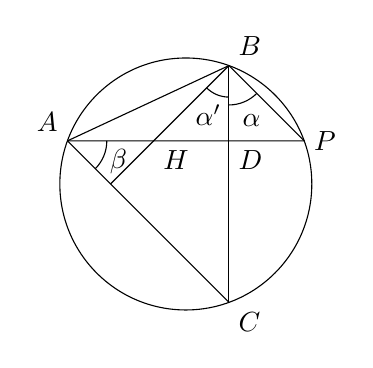
\begin{tikzpicture}[scale=0.8]
			          %projection ($(X)!(B')!(B)$)
			          %nommer chemin 'name path
			          %intersection \path [name intersections={of=d and gb,by=G}];
			          %animation  \draw[visible on=<1>] 
				  %           \draw[visible on=<{2,4}>]
				  %angle arc[radius = 6mm, start angle= 180, end angle= 225] node [below left,pos=0.3]{$\alpha$}
				  %angle \pic [draw, visible on=<2>, above left,"$\beta$", angle eccentricity=1.5] {angle = A'--A--B};
				  %perpendiculaire ($(A')!3cm!-90:(A)$)
				  
				  %CERCLE et triangle
				  \coordinate (O) at (0,0);
				  \coordinate[label=above right:$B$] (B) at (70:2);
				  \coordinate[label=below right:$C$] (C) at (-70:2);
				  \coordinate[label=above left:$A$] (A) at (160:2);
				  \draw[name path =cercle] (O) circle (2);
				  \draw (A) -- (B);
				  \draw (C) -- (A);
				   \draw[name path=BC] (B) -- (C); 
				   
				   %D,P
				   \path[name path =AP] (A) -- +(4,0);
				   \path [name intersections={of=AP and BC,by=D}];
				   \path [name intersections={of=AP and cercle,by=P}];
				   \coordinate[label= below right:$D$] () at (D);
				   \coordinate[label= right:$P$] () at (P);
				   \draw[name path=AP] (A) -- (P);
				   \draw (B) -- (P);
				   
				   %H
				   \draw[name path=BH] (B) -- ($(A)!(B)!(C)$);
				   \path [name intersections={of=AP and BH,by=H}];
				   \coordinate[label= below right:$H$] () at (H);
				   
				   %ANGLES
				   \pic [draw,"$\alpha$", angle eccentricity=1.5] {angle = D--B--P};
				   \pic [draw,"$\alpha '$", angle eccentricity=1.7,angle radius=4mm] {angle = H--B--D};
				   \pic [draw,"$\beta$", angle eccentricity=1.4] {angle = C--A--D};
				   
				  \end{tikzpicture}
				  \end{figure}
			
				  \begin{tcolorbox}[basic] 
				      
				    \smallskip
				    \underline{Hypothèses} 
				    \begin{enumerate}
				    \item $AH$ hauteur issue de $A$,
				    \item $BH$ hateur issue de $B$,
				    \item $\Delta ABC$ inscrit dans un cercle. 
				    \end{enumerate}
							      
				    \underline{Thèse} \\
				    \smallskip
				    $|HD=|DP| $.
				    \end{tcolorbox}
		
		
		\column{.5\textwidth}\centering
		
		\underline{Résolution}\\ \flushleft
		\heart Deux $\Delta$ sont isométriques lorsqu'ils ont un côté de même longueur compris entre deux angles de mêmes mesures. \\ \medskip
		
		\begin{enumerate}
		 \item $\widehat{BDP}=\widehat{BDA}$,
		 \item \begin{align*}
		        \alpha =& \beta, \text{ (angles inscrits)} \\
			       =& \alpha '. \text{ (angles à côtés $\bot$)}      
		       \end{align*}
		\end{enumerate} \medskip
		Côté $[BD]$ en commun. \\ \bigskip
		$\Delta BDH,\Delta BDP$ isométriques. \\ \bigskip
		
		\centering 
		
		$|HD|=|DP|$.  \\
		\hfill $\qed$
		
	   \end{columns}
    
    \notedir{%
	   .1 Prouver thèse.
	   .2 $|HD=|DP|$.
	   .3 Elément de théorie.
	   .4 2 $\Delta$ isométriques ont leurs côtés correspondants de même longueur..
	   .3 Résolution..
	   .4 $\Delta BDH, \Delta BPD$ isométriques car.
	   .5 Chacun un angle droit.~($AD$ est la hauteur)..
	   .5 Côté $[BD]$ en commun..
	   .5 $\alpha=\beta$ (angles inscrits) et $\beta=\alpha'$ (angles  à côtés $\bot$ car hauteurs) $\rightarrow \alpha=\alpha '$..
	   .4 $\Delta BDH, \Delta BPD$ isométriques $\rightarrow |HD=|DP|$.. 
	   }
    }
	  
  
\end{document}
